

\documentclass[a4paper, 12pt]{article}

\usepackage[utf8]{inputenc}



\usepackage[T1]{fontenc}
\usepackage[utf8]{inputenc}
%\usepackage{listings}

\usepackage{amsmath, amssymb, amsthm}
\usepackage{geometry, emptypage}
\usepackage{graphicx, subfig}
\usepackage{enumitem, lipsum}
%\usepackage{marginnote, xspace}
\usepackage{comment}

%\usepackage[autostyle,italian=guillemets]{csquotes}

\usepackage[boxed]{algorithm2e}
\usepackage[eulerchapternumbers, palatino=false, parts=false]{classicthesis}
\usepackage{arsclassica}

\usepackage{setspace}
 \setstretch{1.1}


\usepackage{hyperref}


\usepackage[square,numbers]{natbib}
\bibliographystyle{unsrtnat}

\usepackage{xcolor}

\usepackage{afterpage}
\newcommand\emptypage{
    \null
    \thispagestyle{empty}
    \addtocounter{page}{-1}
    \newpage
    }
    
\usepackage{multicol}



% Font
\usepackage[proportional, oldstyle, scale=1.03]{cochineal}
\usepackage[english]{babel}
\usepackage[varqu,varl,var0]{inconsolata}
\usepackage[scale=.95,type1]{cabin}
\usepackage[cochineal,vvarbb]{newtxmath}
%\usepackage[cal=boondoxo]{mathalfa}



% Figures
\graphicspath{{plots/}}
\captionsetup{format=hang}

% Layout
\geometry{%showframe,
	width=35pc, height=57pc, vmarginratio=1200:1000}
\setlength{\parindent}{0.7em}
%\setlength{\parskip}{0.em}

\newcommand\setupheading[1]{%
	\cleardoublepage\phantomsection
	\markboth{\spacedlowsmallcaps{#1}}{\spacedlowsmallcaps{#1}}%
}


% Headings
\renewcommand{\sectionmark}[1]{
	\markright{\thesection\enspace\textit{#1}}
} 
\clearplainofpairofpagestyles


% Other
\hypersetup{%hidelinks,
	linkcolor=RoyalBlue}
\microtypesetup{kerning=true}
%\let\marginpar\marginnote
\let\bm\boldsymbol
\setlist{itemsep=0pt}



\usepackage[square,numbers]{natbib}
\bibliographystyle{unsrtnat}

%\setlength{\parindent}{4em}
\setlength{\parskip}{0.5em}
\renewcommand{\baselinestretch}{1.1}

\pagenumbering{gobble}


%\geometry{a4paper,top=2.5cm,bottom=2.5cm,left=2.5cm,right=2.5cm}% heightrounded,bindingoffset=5mm


%%%%% AUTHORS - PLACE YOUR OWN COMMANDS HERE %%%%%

% Please keep new commands to a minimum, and use \newcommand not \def to avoid
% overwriting existing commands. Example:
%\newcommand{\pcm}{\,cm$^{-2}$}	% per cm-squared

% quick alias
\def\be{\begin{equation}}
\def\ee{\end{equation}}
\newcommand\code[1]{\textsc{\MakeLowercase{#1}}}
\newcommand\quotesingle[1]{`{#1}'}
\newcommand\quotes[1]{``{#1}"}
\def\gsim{\lower.5ex\hbox{\gtsima}} 
\def\lsim{\lower.5ex\hbox{\ltsima}} 
\def\gtsima{$\; \buildrel > \over \sim \;$} 
\def\ltsima{$\; \buildrel < \over \sim \;$} \def\gsim{\lower.5ex\hbox{\gtsima}} 
\def\lsim{\lower.5ex\hbox{\ltsima}} 
\def\simgt{\lower.5ex\hbox{\gtsima}} 
\def\simlt{\lower.5ex\hbox{\ltsima}} 


% solar stuff units
\def\msun{{\rm M}_{\odot}}
\def\lsun{{\rm L}_{\odot}}
\def\dsun{{\cal D}_{\odot}}
\def\fsun{\xi_{\odot}}
\def\zsun{{\rm Z}_{\odot}}
\def\msunyr{\msun/{\rm yr}}
% units
\def\mum{\mu {\rm m}}
\newcommand{\angstrom}{\mbox{\normalfont\AA}}
\def\cc{\rm cm^{-3}}
\def\kms{\,\rm km\,s^{-1}}
\def\kpc{\,\rm kpc}
\def\uflux{{\rm erg}\,{\rm s}^{-1} {\rm cm}^{-2} }
% quantities defs
\def\fdust{\xi_{d}}
\def\fesc{f_{\rm esc}}
\def\td{\tau_{sd}}
% additional wrappers for quantities and units
\def\Dsolar{${\cal D}/\dsun$}
\def\Zsolar{$Z/\zsun$}
\def\DDsolar{\left( {{\cal D}\over \dsun} \right)}
\def\ZZsolar{\left( {Z \over \zsun} \right)}

% LINES
\def\S*{$\Sigma_{\rm SFR}$}
\def\Scii{$\Sigma_{\rm CII}$}
\def\Sciimax{$\Sigma_{\rm CII}^{\rm max}$}
\def\CII{\hbox{[C~$\scriptstyle\rm II $]~}}
\def\CIII{\hbox{C~$\scriptstyle\rm III $]~}}
\def\OIII{\hbox{[O~$\scriptstyle\rm III $]~}}

%\def\CII{[CII]~} 
%\def\CIII{CIII]~}
% IONS
\def\HH{\hbox{H$_2$}~} 
\def\H{\hbox{H}} 
\def\He{\hbox{He}} 
\def\HI{\hbox{H~$\scriptstyle\rm I\ $}} 
\def\HII{\hbox{H~$\scriptstyle\rm II\ $}} 
\def\HeI{\hbox{He~$\scriptstyle\rm I\ $}} 
\def\CIion{\hbox{C~$\scriptstyle\rm I $~}}
\def\CIIion{\hbox{C~$\scriptstyle\rm II $~}}
\def\CIIIion{\hbox{C~$\scriptstyle\rm III $~}}
\def\CIVion{\hbox{C~$\scriptstyle\rm IV $~}}
\def\CVIion{\hbox{C~$\scriptstyle\rm VI $~}}
\def\OIIIion{\hbox{O~$\scriptstyle\rm III $~}}
\def\NIIion{\hbox{N~$\scriptstyle\rm II $~}}

% ion variables
\def\nhh{n_{\rm H2}}
\def\nhi{n_{\rm HI}}
\def\nhii{n_{\rm HII}}
\def\fhh{x_{\rm H2}}
\def\fhi{x_{\rm HI}}
\def\fhii{x_{\rm HII}}
% MIX
\def\fd{f^*_{\rm diss}} 
\def\ks{\kappa_{\rm s}}

% COLORS
\def\cyan{\color{cyan}}
%\definecolor{epcolor}{HTML}{b3003b}
 % definitions.tex contains general used user defined alias and definitions

\renewcommand{\d}{\mathrm{d}}
\newcommand{\der}[3][]{\frac{\d ^{#1}#2}{\d {#3}^{#1}}}
\newcommand{\pder}[3][]{\frac{\partial ^{#1}#2}{\partial {#3}^{#1}}}
\let\oldnabla\nabla
\renewcommand{\nabla}{\vec{\oldnabla}}
\newcommand{\lap}{\oldnabla^2}

\newcommand{\red}[1]{{{\textcolor{red}{\textbf{#1}}}}}
 % math-heavy alias



\begin{document}


%\thispagestyle{plain}
\begin{center}
\vspace{3cm}
    \textbf{{\Large
    Galactic outflows and their role in high-z extended halos formation}
    }    
    
    \vspace{0.5cm}
    \large
    Elia Pizzati
    \vspace{0.5cm}
    
\textit{Supervisors}

\end{center}        


    \begin{multicols}{2}

    \hspace{15mm}{\large Prof. Andrea Ferrara}
    
        \columnbreak
        
    \hspace{10mm}{\large Dr. Andrea Pallottini}
    
    \end{multicols}

       
    \vspace{0.3cm}
\begin{center}
    \textbf{{Extended Summary}}
\end{center}

Investigating the complex environments of galaxies at the end of the Epoch of Reionization (for a recent review see \cite{Dayal:2018hft}) is one of the most pressing research goals of modern astrophysics. As shown by cosmological simulations \citep{fire2, Vogelsberger:2019ynw, sphinx, Pallottini22}, galaxies in the EoR show different properties with respect to the ones seen in the local Universe (e.g., smaller sizes, higher specific star formation rates, warmer dust). Unraveling how galaxies formed and evolved during these remote epochs (i.e., a few hundred million years after the Big Bang) is at the heart of our understanding of cosmic evolution.

In the last few years, astounding progress has been made in detecting these primordial galaxies. This has fueled a strong and widespread interest in detailed studies of their internal structure. As a result, these early systems are now being routinely identified in large-scale Near-Infrared (NIR) surveys  \citep{refId0, bouwens_15}, and targeted interferometric observations at Far-Infrared (FIR) wavelengths \citep{Fevre:2019thf, bouwens_rebels}.

Specifically, the Hubble Space Telescope (HST) and the Very Large Telescopes (VLT) measured sizes and morphological properties of high-redshift galaxies at rest-frame ultraviolet (UV) wavelengths \citep{oesch2009structure,Shibuya:2015qfa, bouwens2017z, kawamata2018size}. These studies successfully characterized the evolution of the rest-frame galaxy UV luminosity functions (LFs), star formation, stellar buildup history, and size growth. For the very first time, we have a solid statistical characterization of galactic systems up to $z\approx 10$. 

At the same time, the appearance of the Atacama Large Millimeter/submillimeter Array (ALMA) and the NOrthern Extended Millimeter Array (NOEMA) have opened a new window on the primordial Universe, exploring the obscured star formation and interstellar medium (ISM) line emission at rest-frame FIR wavelengths up to $z\approx7$. Combining the information coming from the dust continuum emission, as well as from some relevant FIR emission lines such as \CII $158 \,\mu\mathrm{m}$, \OIII $88 \,\mu\mathrm{m}$, and CO from various rotational levels, several works studied the internal properties of galaxies, such as their assembly history, ISM thermal structure, gas dynamics, dust/metal enrichment, and interstellar radiation field (ISRF) \citep{maiolino2015,capak2015,pentericci2016, matthee2017, carniani2018,Hashimoto2018, gallerani:2018}.


The data coming from this plethora of observations can be compared to state-of-the-art, zoom-in cosmological simulations \citep{pallottini2017, Hopkins18, pallottini:2019}. In doing so, on one hand, we can benchmark the results of simulations and assess the physical assumptions on which they are based, and on the other hand, we can search in observational data for the features expected from theoretical considerations. One of the most important predictions made by cosmological simulations is known as the \textit{baryon cycle} \citep{peroux2020cosmic}. This process describes the history of baryons in the galactic environment, taking account of the complex interplay between star formation, stellar feedback, and accretion from the circumgalactic medium (CGM). Baryons are brought to great galactocentric distances ($1-100\,\mathrm{kpc}$ scales at $z\approx 6$) by feedback mechanisms, but, at the same time, they are also accreted to the inner region of the galaxy due to the gravitational influence of the dark matter halo. Simulations clearly reveal how this process is responsible for driving galaxy growth \citep{tumlison}. Therefore, understanding the physics behind the competing processes of outflowing and inflowing matter is a key step to improve our understanding of cosmic evolution \citep{2005ARA&A..43..769V}.

Signs of galactic outflows were first found at low redshift a few decades ago \citep{chevalier_clegg:1985, Walter:2002vq}, but only very recently there has been strong evidence of the presence of outflows in high redshift galaxies. Outflows were seen in massive quasar-hosting galaxies \citep{cicone2015}, as well as in normal star-forming ones \citep{gallerani:2018, ginolfi:2019, Sugahara19, herrera2021kiloparsec}, suggesting their ubiquitous presence and supporting the claim that they steer galaxy evolution from the EoR to the present day \citep{veilleux2020cool}. 

However, despite the remarkable improvements made both from theoretical and observational perspectives, we are still lacking a deep and thorough description of the outflows driving mechanisms, and of their morphological, thermal, and chemical structure \citep{heckman2017galactic}. Both observations and detailed simulations suggest that outflows present a complex multi-phase structure \citep{murray2011, hopkins2014, muratov2015,pandya2021characterizing}. These phases often coexist together in the outflow, sharing the energy and mass budgets of the outflowing gas. Moreover, hot gas can turn into a cold mode by emitting radiation and thus cooling down to a lower temperature via \textit{catastrophic radiative cooling}. This process can start when the threshold for H, He, and metal lines cooling is reached, and it rapidly lowers the temperature of the gas by several orders of magnitude. Different works highlight the role of this catastrophic cooling in regulating feedback mechanisms in super-star clusters \citep{Silich:2004,gray2019catastrophic} and galaxies \citep{Wang:1995, sarkar:2015, Thompson16, Schneider:2018, Gronke&Oh:2020}. Nevertheless, the role of this physical process in real cosmological environments is yet to be characterized properly.

Another important piece of the puzzle comes from recent observations of the circumgalactic medium (CGM) of $z\approx4-7$ galaxies. Several studies hint at the presence of singly ionized carbon surrounding these primeval galaxies \citep{Fujimoto19, Fujimoto:2020qzo, ginolfi:2019, herrera2021kiloparsec}. Using ALMA measurements of the \CII line emission, they show that carbon extends out to a distance ($\sim 10-15 \,\mathrm{kpc}$) that is significantly larger than the size of the galaxy itself, creating an \textit{extended halo} that dominates the properties of the galaxy's CGM. The first statistically significant evidence for such halos was obtained by \citet{Fujimoto19} via stacking of $z\approx6$ galaxies. This study was then backed up by detailed individual observations within the ALMA ALPINE Large Program \citep[][]{lefevre:2019, Fujimoto:2020qzo}. On top of these findings, observations of single systems such as lensed dusty star-forming galaxies \citep{Rybak20} also found signs of extended \CII emission arising in the outskirts of the galaxy. 

The mounting observational evidence for the existence of extended \CII halos at high redshift inevitably calls for a thorough theoretical investigation of their origin, properties, and connection with the CGM/IGM surrounding primeval galaxies. A direct comparison with mock observations generated by using $z=6$ zoom simulations \citep{pallottini2017b, Arata:2019}, however, fails to reproduce the observed \CII surface brightness distribution of the emitting material in extended halos \citep{Fujimoto19}.

These independent studies agree in predicting a \CII emission that is slightly more extended than the stellar continuum but drops very rapidly at distances considerably smaller than $10\,\mathrm{kpc}$. This mismatch between theory and observations could originate either from issues in modelling FIR emission lines or because of some key physical ingredients that are still missing or not well captured by simulations. In any case, however, such tension represents a serious challenge in our understanding of early galaxy formation. 

This Thesis aims at taking on the problem of finding plausible mechanisms to explain the formation of these halos. In particular, we connect all the pieces of evidence here presented, focusing on the hypothesis that these halos result from the remnants of past -- or ongoing -- outflow activity. We explore this idea by using a semi-analytical model for an outflow that undergoes \textit{catastrophic cooling} in the inner region of the halo. The goal of our exploratory work is to bridge the gap between simulations and observational data, by employing our framework to explore the physical implications of the observed emission and put the development of new simulations on the right track.

The model we develop builds on previous studies of galactic winds \cite{chevalier_clegg:1985, Thompson16}. We model the galaxy active star forming region as a sphere of radius $R=300\,\mathrm{pc}$. Energy and mass are uniformly injected from this region at a constant rate to mimic the input of supernovae (SN) associated with the star formation activity. This energy and mass deposition drives a spherically symmetric, and steady wind that expands freely in the region outside the galaxy (the presence of the IGM/CGM is neglected). We consider the mass loading factor, $\eta$, as a key parameter in our model, as it dictates the initial thermodynamic properties of the gas.

Radiative losses are included in the model by introducing the net (i.e., cooling--heating) cooling function $\Lambda$, taken from the Tables in \citet{gnedin2012cooling}. Rapid cooling plays a key role in our formulation, as the formation and survival of \CII in the gas is guaranteed only for relatively low temperature values ($T\lesssim 10^4\,\mathrm{K}$). Along with cooling, it is also important to consider the gravitational effects of the galaxy's dark matter (DM) halo on the gas. This is because, as the gas cools down radiatively, it slows down considerably, and thus its velocity becomes comparable with the escape velocity from the galactic system. The gravitational pull acting on the wind depends in our parametrization on the halo circular velocity $v_c$. 


Since we assume photo-ionization equilibrium (PIE), the cooling (and heating) rates are strongly dependent on the ionizing radiation fields impinging on the gas. In turn, these fields can be produced either by leakage of ionizing photons from the parent galaxy, or by the cosmological contribution from all the other galaxies and quasars (the UV background, UVB). We include both these contributions in the model, parametrizing the former via the escape fraction of ionizing photons from the parent galaxy ($\fesc$).


With this set of assumptions, a cool (i.e., $10^2\,\mathrm{K}\lesssim T \lesssim 10^4\,\mathrm{K}$) wind that drives carbon (and supposedly other metals) into the CGM of the galaxy can be obtained (Figure \ref{fig:profiles}). The wind is slowed down by the gravitational potential, and reaches a stalling radius $r_\mathrm{stop}$ at distances comparable with the sizes of the observed \CII halo \citep[][]{Fujimoto19}. 


The thermodynamic properties of the outflow are then used, along with the hypothesis of photo-ionization equilibrium, to compute the abundance of neutral hydrogen and \CIIion in the gas. The relative amount of Carbon and other metals in the gas is set to solar values, in accordance with the results of simulations at $z\approx6$ \citep{pallottini2017, pallottini:2019} and with the extrapolation of the mass-metallicity relation at high redshifts \citep{mannucci:2012}. Together with the outflow temperature and density, relative abundances of $\HI$ and $\CIIion$ determine the emissivity of the \CII line. Assuming that this line is optically thin, a straightforward line integration holds the \CII surface brightness distribution: this is the final quantity that can directly be compared with the observed distributions of \CII extended emission. Note that a fair comparison with observations can only be achieved by correcting the \CII line emissivity for the effects of the Cosmic Microwave Background (CMB) suppression, which is important for the \CII line at high redshift \cite{gong2012, dacunha2013, vallini2015, kohandel:2019}.

Overall, our model makes quantitative predictions on the properties of a \CII halo generated by outflowing gas from a galaxy. It takes as inputs some key parameters, such as the outflow mass loading factor ($\eta$), the parent galaxy star formation rate ($\mathrm{SFR}$) and the escape fraction of ionizing photons ($\fesc$), and the circular velocity of its dark matter (DM) halo ($v_c$). We find that our model outputs are in very good agreement with observations \citep{Fujimoto19, Fujimoto:2020qzo} provided that: (a) the outflow mass loading factor $\eta$ is relatively high ($\eta \gtrsim 3$); (b) the escape fraction of ionizing photons from the parent galaxy is very low ($\fesc < 1\%$). The first condition ensures that the density of the outflowing gas is high enough to match the observed \CII surface brightness; the second prevents the galaxy radiation from ionizing the gas in the halo and leaving only trace amounts of \CIIion in the gas. 

We then focus on these promising configurations and study them for seven individual \CII-halo-hosting galaxies observed by the ALPINE survey \citep{Fujimoto:2020qzo}. We run a Markov-Chain MonteCarlo (MCMC) to find the best fit values of the parameters of our model for every single system and characterize the resulting posterior distribution for these parameters (Figure \ref{fig:corner}). Finally, we focus on the implications of our findings in light of previous work on outflows at low and high redshift. In agreement with other theoretical predictions \citep{Finlator:2007mh, muratov2015}, we find that the mass loading factors for high-z, normal star-forming galaxies lie in the range $\eta\approx 4 - 7$, with higher values attained by low-mass/low-SFR systems (Figure \ref{fig:final}).


 
 




\begin{figure*}
    \centering
    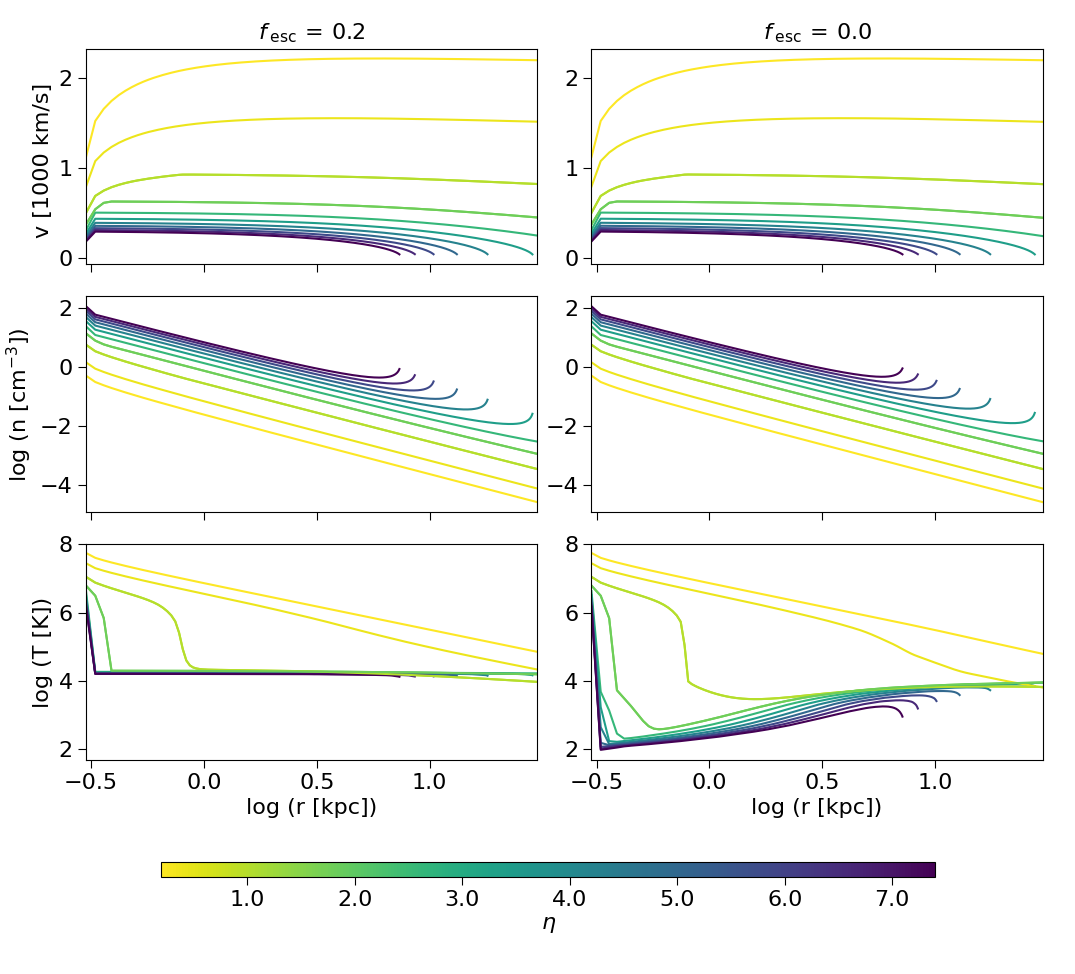
\includegraphics[width=1.\textwidth]{plots/profiles.png}
    \caption{Radial profiles of key outflow thermodynamical variables obtained in an instance of our outflow model. Shown are the results for two different values of the escape fraction of ionizing photons $\fesc=0.2$ (left column), and $\fesc=0$ (right).
    \textit{Top row}: Velocity ($v$). For high values of the mass loading factor $\eta$, gravity slows down the outflow until a stalling radius at which $v=0$ is reached.
    %
    \textit{Middle}: Density ($n$). The radial dependence of the density is generally $n\propto r^{-2}$, but its value increases as the gas slows down due to gravity.
    %
    \textit{Bottom}: Temperature ($T$). Note the rapid transition (for high values of $\eta$) from a hot wind to a cool/warm one due to the presence of catastrophic cooling. After cooling has taken place, the temperature profiles depends on the escape fraction considered: for $\fesc=0$ the outflow cools to even lower temperatures and reaches the equilibrium value of $T\approx10^4\,\mathrm{K}$ only at much larger radii.  
         \label{fig:profiles}
    }
\end{figure*}





\begin{figure*}
	\centering
	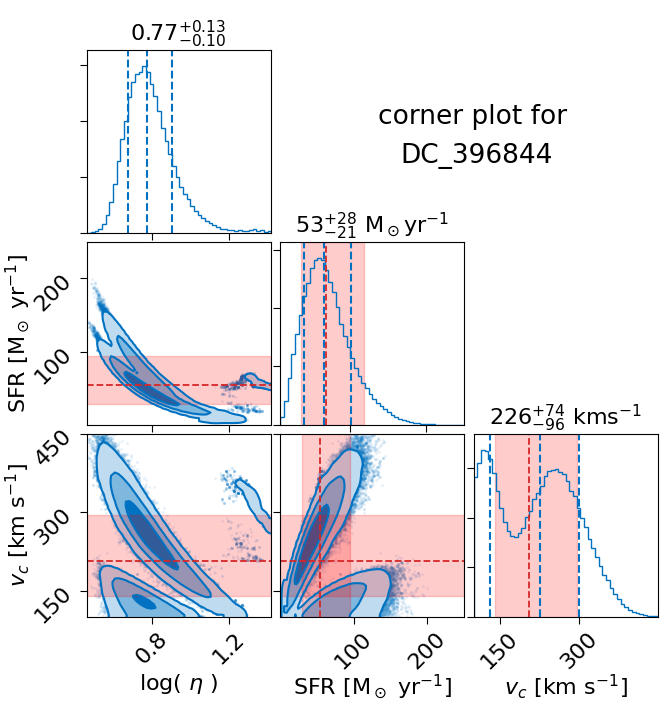
\includegraphics[width=0.495\textwidth]{plots/corner.png}
	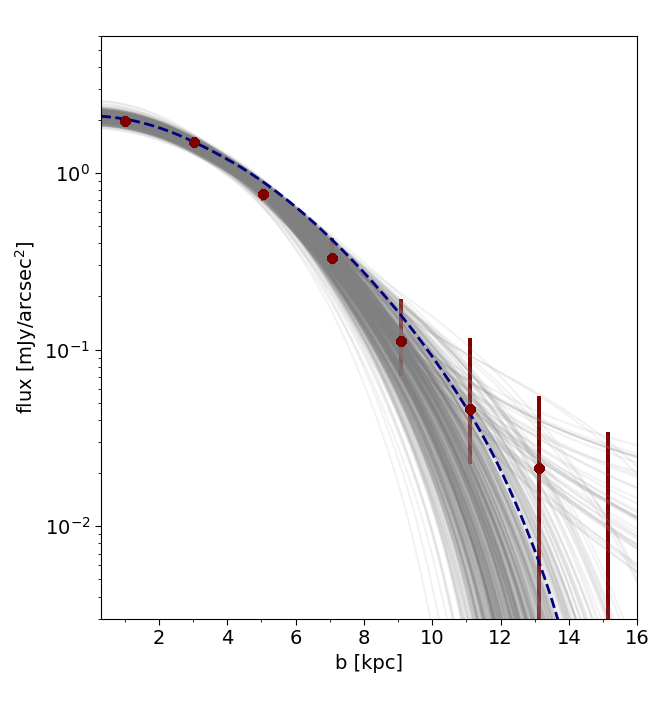
\includegraphics[width=0.495\textwidth]{plots/emission_final_single.png}
	\caption{\textit{Left:}
	%
	Corner plots of the 3D posterior distribution for the galaxy DC$396844$ (taken as an example from our sample of 7 galaxies). The parameters considered bere are: the mass loading factor $\eta$, the star formation rate (SFR) ad the DM halo's circular velocity ($v_c$).
	%
	The values of $\mathrm{SFR}$ and $V_{\rm c}$ inferred from observations are shown with red dashed lines, together with their uncertainties (red shaded regions). The blue dashed vertical lines represent the median values and $1\sigma$ errors on the parameters: these same quantities are also reported at the top of each 1-d histogram.
	%
	\textit{Right}: Comparison of the \CII surface brightness profiles obtained from our model (light gray lines) for the system DC$396844$ with the observed profiles \citep[][red points]{Fujimoto:2020qzo}. The synthesised profiles are created from randomly sampling the posterior distribution $500$ times. The blue dashed line highlights the results for the median values of the parameters (see left panel).
	    \label{fig:corner}
	}
\end{figure*}

\begin{figure*}
	\centering
	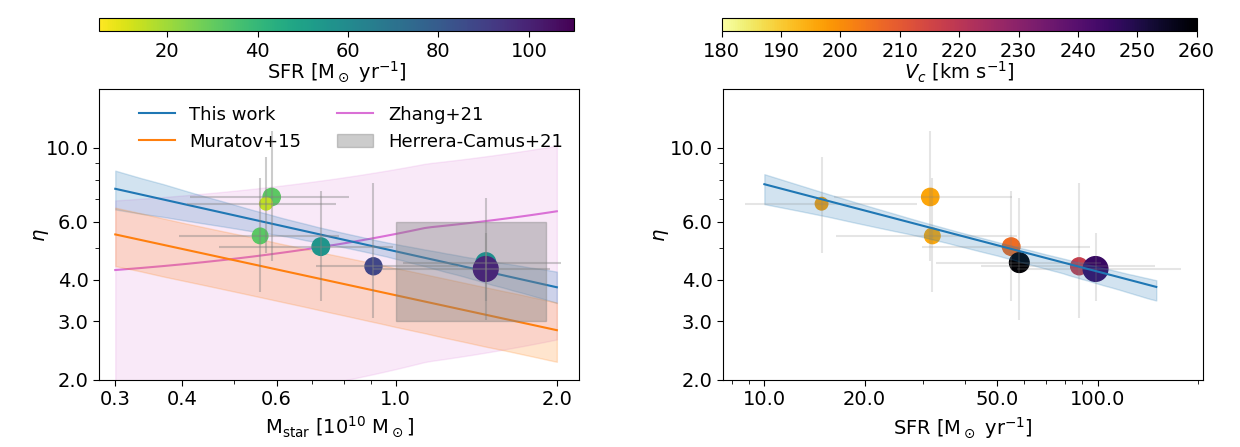
\includegraphics[width=1.0\textwidth]{plots/final_comparison_new_paper.png}
    \caption{\textit{Left}: Dependence of the mass loading factor $\eta$ (shown are median values and associated 1$\sigma$ error) on the stellar mass $M_\mathrm{star}$. Stellar masses are obtained from observational data \citep{Fujimoto:2020qzo}. The blue line show the best power-law fit to the data. For reference we also show predictions from other studies such as \citet[][orange]{muratov2015}, \citet[][purple]{zhang2021empirical}, and \citet[][grey rectangle]{herrera2021kiloparsec}. Data points are color-coded according to their SFR, as inferred from observations. The size of every point is proportional to the value of the likelihood. \textit{Right}: Same as left panel, but for the star formation rate (SFR). The color of the data points corresponds to their virial velocity $V_{\rm c}$ (see colorbar), as inferred from observations.
    \label{fig:final}
	}
\end{figure*}


\newpage
\bibliography{biblio}


\end{document}